\chapter{Integration of rainfall radar data with a landscape evolution model}
\label{chapter_metdata}
\chaptermark{Linking rainfall radar data with LEMs}

%%%%%%%%%%%%%%%%
% TO DO
% 
% Figures of total rainfall accumulation over catcments
% Zoomed in location maps
%
%%%%%%%%%%%%%%%%
%\begin{chapquote}{Claude Monet \textit{}}
%``It's enough to drive one crazy, trying to depict the weather, the atmosphere, the ambience...
%\end{chapquote}

\section{Introduction}
%This chapter discusses the various sources of meteorological data and numerical models used to generate rainfall input to the landscape evolution models discussed in Chapters \ref{chapter_landscape_evol} and \ref{RainfallInLEMs}. In this thesis, two sources of rainfall data were used to drive the hydrological inputs of landscape evolution models: precipitation radar data from the UK 1km rainfall radar composite product (Section \ref{NIMROD}) and rainfall outputs from a numerical weather prediction model (Section \ref{WRF}

Measuring and predicting rainfall has been a central activity to meteorological and hydrological sciences for centuries. The importance of having good estimates of rainfall for understanding hydrological processes was recognised by \citet{perrault1674}, particularly for understanding the role of rainfall in the water cycle \citep{biswas1970history}. Historically, the earliest hydrometeorological observations in Britain were recorded by Bede the Venerable (AD 672--735) \citep{mcculloch1993history}. Quantitative measurement of rainfall with instrumentation in the UK is attributed to Christopher Wren and Robert Hooke \citep{biswas1970history}, who developed a precursor to the modern tipping-bucket raingauge, although numerous records of rainfall measurement have been noted in other societies predating efforts in Britain \citep{strangeways2010history}. Quantifying the amount of rainfall that has fallen in a given area over a period of time is referred to formally as \textit{quantitative precipitation estimation} \citep{fabry2015radar} and its prediction ahead of time as \textit{quantitative precipitation forecasting} \citep{golding2000quantitative,browning2003quantitative}.

In the context of landscape evolution and erosion modelling, realistic rainfall input sources are often a secondary consideration, with many models using a uniform rainfall rate across the model domain, or generating rainfall inputs artificially from stochastic rainfall generators \citep[Chapter \ref{chapter_RainfallInLEMs},][]{Tucker2000}. Despite the paucity of realistic rainfall data use in landscape evolution modelling, there is no shortage of rainfall data at the disposal of the landscape evolution modeller. This chapter explores some of the potential meteorological data sources that could be incorporated into numerical models of landscape erosion and evolution, and presents a software framework for processing rainfall radar data for use in the CAESAR-Lisflood landscape evolution model, and its derivative models.

\subsection{Rainfall data sources}
% Raingague
Direct measurement of rainfall is accomplished through the use of rainfall gauges, which provide in situ measurement of rainfall totals, and in some cases, instantaneous rainfall rates, at a fixed-point location. In the UK, the density and spacing of rainfall gauges is heterogeneous at the individual catchment scale, though there is good coverage at regional to national scale. At catchment and sub-catchment scale, however, most rainfall gauge networks are too sparse to provide detailed information about the distribution of rainfall variability within a catchment. Exceptional coverage is sometimes found in catchments that have been instrumented as `research catchments', where a high-density network of gauges has been established for monitoring of specific catchments, \citep[e.g. the Plynlimon research catchment,][]{newson1979results} but this is atypical. Though raingauges are reliable for point totals of rainfall, common types of gauge (such as the widespread tipping-bucket raingauge) have a tendency to underestimate true rainfall rates during very high rainfall intensities \citep{habib2001sampling,ciach2003local}. Nonetheless, the rain gague data is used extensively for verifying and calibrating other indirect measurements of rainfall, such as satellite or radar \citep{harrison2000improving,ebert2007methods}, or predictions from numerical weather forecast models \citep{golding2000quantitative}.

%Satellite
Indirect measurements of precipitation can be either \textit{active} or \textit{passive} in their mode of measurement. Active sensors emit a pulse of electromagnetic radiation, usually in the microwave--radiowave band depending on the application, and measure the amount of energy reflected back from hydrometeors \citep{fabry2015radar}. A mathematical function is used to convert the measurement of reflected electromagnetic radiation into a rainfall rate or rainfall amount, the choice of function depending on the particular method used. Passive sensors, as their name implies, do not actively emit any kind of electromagnetic radiation directly, but measure only the radiation emitted naturally from the Earth's surface. When precipitation is present over the surface, passive sensors measure the brightness temperature\footnote{Brightness Temperature is a descriptive measure of radiation in terms of the temperature of a hypothetical blackbody emitting an identical amount of radiation at the same wavelength.} from the surface, and use this measurement to determine the phase and intensity of rainfall present based on a number of physical and empirical conversion formulae. Many satellite precipitation measurement missions combine active and passive sensing to build a complete picture of rainfall on the Earth's surface (e.g. the \textit{Tropical Rainfall Measurement Mission}, TRMM, \citet{simpson1988proposed}, the \textit{Global Precipitation Measurement Mission}, \citet{hou2014global}). The advantage of satellite precipitation measurements lies in their ability to cover large regions of the globe, which would be infeasible with a network of ground-based measurements. Satellite precipitation measurements are particularly useful at increasing the coverage of rainfall measurement over the oceans, where there is a particular paucity of other measurement sources. Limitations in satellite precipitation measurement include its lower resolution compared to ground based measurements, due to the distance between the surface and the orbiting sensor, as well as the lack of coverage around polar regions on most satellites. Due to the orbiting nature of satellites, they cannot currently take measurements with the same frequency as ground-based methods. Typical temporal resolution of satellite measurements is on the order of 1.5--3 hours, whereas ground-based methods can take measurements up to every few minutes. Consequently, space-borne measurements are not usually suitable for applications requiring high-frequency, high-resolution measurements of rainfall, but lend themselves well to providing consistent, near-global coverage (with the exception of polar regions). 

%Radar
Ground-based precipitation radars are active sensors, emitting pulses of electromagnetic radiation in a 360\degree \ field of view through a rotating antenna. They measure the intensity of the beam that is reflected and use this to derive a rainfall rate through a series of empirical formulae \citep{wilson1979radar}. The scanning beam is angled slightly above level (typically 5\degree) allowing a near-surface measurement of rainfall at close range, which gradually becomes higher as the beam extends in range.  Rainfall radars have a large variety of ranges depending on application, but national weather service radar stations typically have a range of 200--500 km in diameter \citep{fabry2015radar}.  

\subsection{Advantages of radar for hydrological applications}
Weather radar is particularly well suited to use in hydrological applications, and for the purposes of this thesis, by extension, to landscape erosion models that feature a hydrological component. There are two principal hydrological applications \citep{harrison2012radar}: 1) routine monitoring of precipitation for climatological data collection, day-to-day river management, weather forecasting, and model validation; 2) early detection and prediction of floods for civil protection purposes. Both applications have common requirements such as data accuracy, but early flood detection has the added need for rapid estimation and dissemination of rainfall rates in order to give as much lead time as possible to authorities responsible for flood prediction and mitigation \citep{fabry2015radar}. 

Rainfall radar is particularly useful in small catchments, where response times to intense rainfall events are short, and where rapid rises in river level can quickly overcome infrastructure such as flood defences, reservoirs, and dams. With smaller catchments, the likelihood of having other sources of rainfall and hydrological information diminishes, such as rainfall and river flow gauges \citep{fabry2015radar}. In larger catchments with adequate gauging facilities, precipitation may have large variability in spatial patterns, necessitating the use of other methods to determine the distribution of rainfall inputs into a river catchment. Large, mountainous catchments also benefit from rainfall radar as they may experience intense localised rainfall and quickly channel the rain from steep hillslopes into gorges and river channels.



\subsection{Basic principles of Radar}

Radar works on the principle of emitting microwaves and measuring the intensity and time taken of waves reflected back from distant hydrometeors. The use of radar to detect distant rainfall was alluded to by \citet{marshall1947measurement} who wrote: 

\begin{quotation} 
``\textit{It may be possible therefore to determine with useful accuracy the intensity of rainfall at a point quite distant (say 100km) by the radar echo from that point}".
\end{quotation}

The basic principle of rainfall radar remains the same to this day, though technological advances have increased the quality and speed of dissemination of rainfall measurements. Specifically, meteorological radar measures the reflectivity, and uses this value to determine the intensity of rainfall through an empirical formula relating reflectivity intensity to a rainfall rate. This is refereed to as the Z--R relationship, where \(Z\) is the reflectivity and \(R\) is the rainfall rate. Many variants of the formula exist, taking the general form of:
  
\begin{equation}
Z = aR^b
\end{equation}

\noindent
where \(a\) and \(b\) are empirically-derived constants \citep{gunn1949terminal,joss1969raindrop}.

\subsection{Processing and error correction}

The reflectivity returns measured at any individual radar site are a combination of the radar waves reflected off hydrometeors at the scan level at a given moment in time, plus any other objects or obstacles in the path of the radar, plus a level of background noise from the atmosphere and instrument. From receiving raw radar return signals, there follow several steps to process this data and convert it into a usable rainfall product, giving an accurate estimate of surface rainfall. Post-processing steps can be summarised as follows:

\begin{enumerate}
\item Noise removal. Background noise may come from instrumental sources or sources in the atmosphere. A typical approach to noise removal is to estimate the mean noise from scans take on precipitation-free periods and subtract this from the measured return reflectivity.

\item Removal of non-precipitation echoes. Sources of non-precipitation echoes include insects, birds, air and shipping traffic, and interference from other radar emitters. There are several approaches to removing this type of echo, some combining several techniques into one \citep{germann2006radar,rico2008classification}.

\item Removal of blocking obstacles such as terrain. Radar scans made at low elevations suffer from blocking of the emitted signals by topography. The effects of blocking on radar reflectivity can be modelled using a high resolution digital elevation map and a model of radar beam propagation \citep{pellarin2002hydrologic}. Another approach is to use long term records of reflectivity and rainfall rate to extrapolate rainfall rates in the blocked regions.

\end{enumerate}

\section{Rainfall radar in Britain and Ireland}

Britain and Ireland are covered by a network of C-band (5 cm wavelength) radar stations. Fifteen of these stations are located in the UK and maintained by the UK Met Office, two in Ireland are maintained by Met {\'E}ireann. A further radar is located on the island of Jersey, maintained by Jersey Met. Combined, these sites give coverage of the whole of Britain, Ireland, and surrounding waters (Figure \ref{fig_radar_map}). The scanning pattern of the radar network returns radar reflectivity data at four elevations every five minutes, at a resolution of 600 m by 1\degree, extending to 250 km in range \citep{harrison2012radar}. 



\begin{figure}[htb]
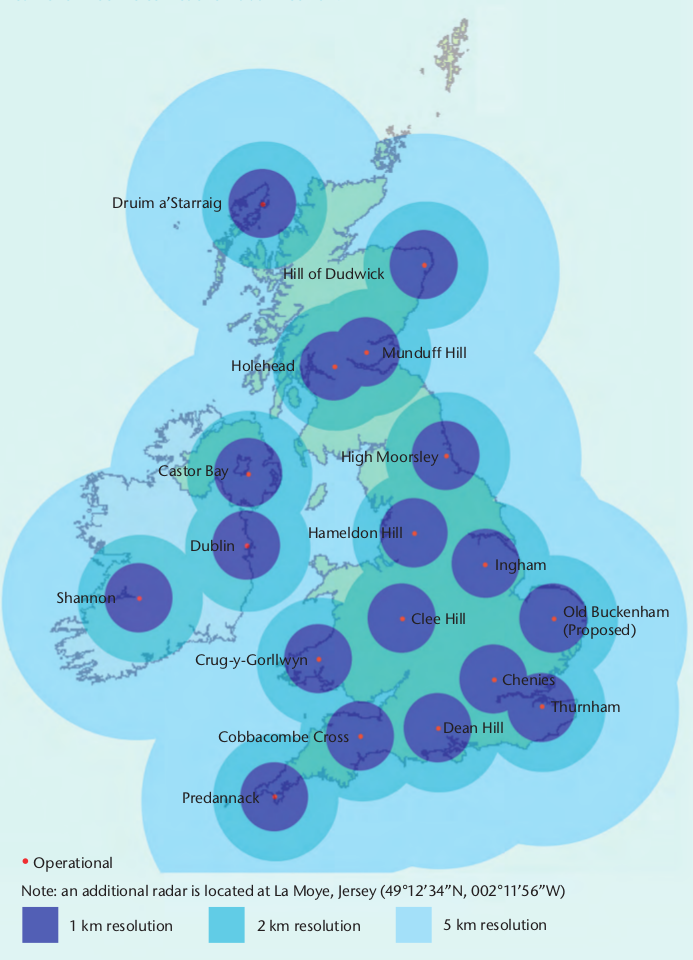
\includegraphics[width=11cm]{chp_radar/radar.png}
\caption{Network of weather radar stations in the British Isles and Ireland. \textit{Source: National Meteorological Library, Met Office, UK.}}
\label{fig_radar_map}
\end{figure}


\section{UK 1km Radar Composite Product}
After processing and error correction of raw radar returns, the rainfall data still exist in a non-gridded format for each individual radar site and the surrounding scan-area. This intermediate format is unsuitable for many applications in environmental modelling and climatology, as adjacent radar sites may report different rainfall rates at locations covered by the overlap of neighbouring radar coverages. To produce a national-scale gridded rainfall data product for the UK, single-site rainfall estimates are composed into a unified data product with a domain covering 47$^{\circ}$--62.7$^{\circ}$N, 13.47$^{\circ}$W--4$^{\circ}$E \citep{metoffice2003nimrod}. Where grid points are covered by overlapping rainfall estimates, the radar with the highest `quality index' -- a function based on the height of the lowest usable radar scan -- is used in the composite data product \citep{harrison2009high}. Other approaches for generating composite radar data products use weighted inputs based on the quality of all radars that provide coverage for a given location \citep{peura2007using}. The finalised UK radar composite product consists of five-minute data at 1 km grid spacing on a regular Cartesian grid. The data is supplied in a proprietary binary format and requires further data processing for ingestion into other models or subsequent analysis. %The code developed to convert this is shown in Appendix 

\section{Use in landscape evolution models}
No currently available landscape evolution models have the capability to directly ingest spatially variable rainfall data from meteorological data sources, such as radar composite products or rainfall data from numerical weather prediction model output. This was a key limitation of current landscape evolution models identified in Chapter \ref{chapter_RainfallInLEMs}. The CAESAR-Lisflood model is capable of ingesting spatially variable rainfall data, but not directly from meteorological data formats, though previous efforts have been made to manually process radar data for the CAESAR-Lisflood model using GIS (Geographic Information System) software \citep[e.g.][]{coulthard2016sensitivity}. The current lack of an automated framework for processing gridded meteorological data for landscape evolution modelling studies substantially slows down research workflows and brings the potential for introducing error or inconsistency between similar studies. Current best-practice advice is to devise automated tools to ensure data processing workflows are reproducible \citep{wilson2014best}.

\subsection{Linking gridded rainfall data with the CAESAR-Lisflood model}
A software framework is presented for processing gridded meteorological rainfall data for ingestion into a landscape evolution model.

Radar data from the UK 1 km composite data product is provided in binary format covering the whole UK \citep{metoffice2003nimrod}. To extract the data for the study area and convert it to a suitable format for the CAESAR-Lisflood model, a further series of post-processing steps are required. The required inputs to the CAESAR-Lisflood model for spatially variable rainfall are:

\begin{itemize}
\item A \textbf{hydroindex grid} file used to mark zones of the catchment that receive different amounts of rainfall throughout the simulation. The hydroindex file has the same dimensions and grid-cell size as the main input terrain DEM in the model.
\item A \textbf{rainfall timeseries} file. This file lists the rain rate at each time step (by row) for each one of the hydroindex zones (by column).
\end{itemize}

The workflow for producing these input files from the radar composite product is:
\begin{enumerate}
\item Convert the composite data from binary format to a human-readable text format.
\item Crop and extract the set of radar images for the time period and geographical extent required. (Figure \ref{fig_radar_extract}.)
\item From the extracted radar images, compile the rainfall rate timeseries. The number of `hydroindex zones' corresponds to the number of radar pixels in the extracted radar data subgrids. (Figure \ref{fig_hydroindex} a.)
\item Produce the hydroindex file at the correct grid-spacing, dimension, and geographical extent. (Figure \ref{fig_hydroindex} d.)
\end{enumerate}

Details of how to access the code for the radar data processing software are given in Appendix \ref{appendix_software}.

\begin{figure}[htb]
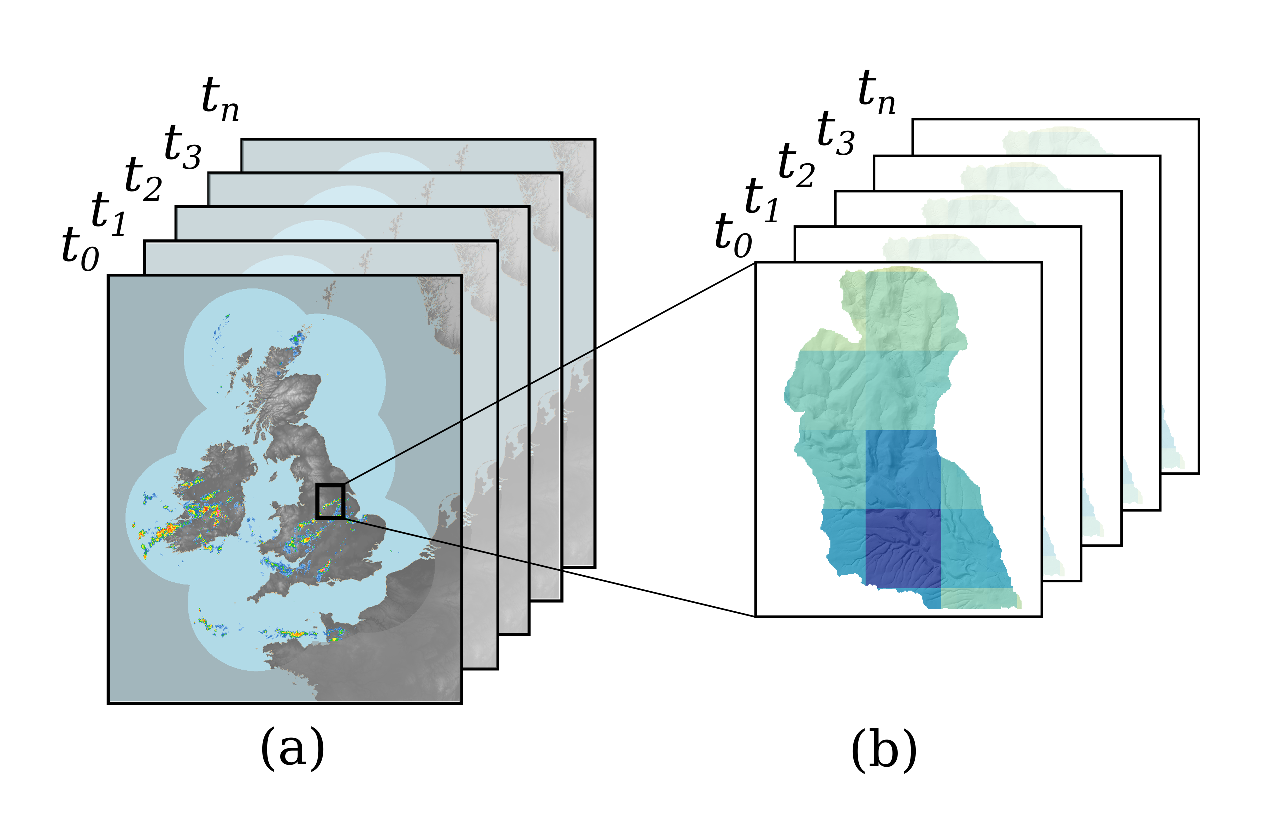
\includegraphics[width=15cm]{chp_radar/cropradar.eps}
\caption{From the UK composite radar product (a), subgrids of the study area extracted for the time period of interest (b). The number of radar image pixels in each subgrid determines the number of hydroindex zones used in the model initialisation.}
\label{fig_radar_extract}
\end{figure}

\begin{figure}[htb]
\includegraphics[width=11cm]{chp_radar/hydroindex.eps}
\caption{(a) Using the extracted radar data subgrids, a timeseries file is created mapping each radar image pixel to a hydroindex zone, for every time step. The hydroindex grid file must be the same dimensions and grid-spacing as the input terrain DEM (b). Numbering each radar image pixel in one of the extracted subgrids (c), the hydroindex file (d), is created from mapping the pixel indexes to the same resolution grid as the terrain input DEM.}
\label{fig_hydroindex}
\end{figure}


\section{Summary}
Rainfall radar is one of many potential sources of rainfall data that can be incorporated with landscape evolution models. Rainfall radar data has several advantages that make it appropriate for use in combination with lansdcape evolution modelling, particularly the CAESAR-Lisflood model. Both model and data source are based on regular, square gridded domains, which makes the translation of rainfall data source to the model input relatively straightforward. The use of other numerical models based on irregular grids, such as the CHILD model,  \citep{Tucker2001}, would require further interpolation steps at the data preparation stage, and possibly at model runtime if the model domain permits adaptive re-meshing \citep{clevis2006simple, tucker2001child}. The CHILD model for example allows the density and location of model grid points to be re-calculated during a simulation to better resolve transient geomorphological features such as river meanders or braided rivers. Fixed gridded models such as CAESAR-Lisflood do not require any grid re-meshing during the model simulation, and the computational costs are potentially reduced for this reason.

For studies using multiple sites and case studies, having a single data source such as a national composite radar product provides a degree of comparability between different sites over different time periods, though upgrades to radar equipment and post-processing algorithms \citep[e.g.][]{harrison2012radar} may negate this advantage if there are large time gaps between case studies, or for long-term studies using rainfall radar data. Rainfall radar's availability in gridded format, and its national coverage availability for the UK since 2004 make it an ideal source of rainfall input data for hydrological and landscape evolution modelling studies. 

The processing framework presented in this chapter provides an automated and reproducible method for extracting sub-regions of gridded rainfall data from the UK 1km composite radar data product and preparing it for ingestion into the CAESAR-Lisflood landscape evolution model and its derivative models.


%
%Rainfall radar are used to infer the spatial distribution and intensity of rainfall over a spatial range of up to several hundred kilometres. Electromagnetic radiation in the microwave spectrum is emitted in pulses through radar antenna that focuses them into a narrow directional beam. When the microwaves encounter hydrometeors (or other obstacles in the path of the beam), the reflected microwave beams are backscattered towards the radar dish. The location and intensity of precipitation can then be calculated using the time taken for the returned radar waves to reach the radar dish, and the amount of backscattered microwave radiation. Radar rainfall measurements are not direct measurements of rainfall, rather they are inferred by making a series of assumptions of how the radar backscatter -- the radar reflectivity -- relates to the quantity and other characteristics of hydrometeors. The amount of radar reflectivity is determined by the size, shape, composition, and distribution of hydrometeors that are sampled by the focused radar beam. Radar reflectivity, denoted by \(Z\), is related to the rainfall rate, \(R\), by the formulation:
%
%\begin{equation}
%Z = aR^b
%\end{equation}

%\section{Numerical Weather Prediction - the Weather Research and Forecasting model}
%\label{WRF}

%Numerical weather prediction models (NWP) are used to predict 
